% \section{Algoritmi di approssimazione}

\section{Introduzione}
% Recap problemi di ottimizzazione, pag 42.

\subsection{Problemi di ottimizzazione}
% pag 5

I problemi di ottimizzazione sono definiti su insiemi di istanze e soluzioni $
\bi, \bs
$ per cui esiste una funzione di costo
% In un problema di ottimizzazione, si definisce una funzione di costo associato ad una soluzione:
\begin{equation*}
    c : \bs{} \to \mathbb{R}
\end{equation*}
e, dato l'insieme di soluzioni ammissibili associate ad un'istanza
\begin{equation*}
    \bs{} (i) = \left\{ s \in \bs{} : i \, \bpi{} \, s \right\}
\end{equation*}
si vuole individuare la soluzione di costo massimo (o minimo)
\begin{equation*}
    s_{i}^{*} = \argmax \left\{ c(s) : s \in \bs{} (i) \right\}
\end{equation*}

\subsection{Approcci risolutivi}

\subsubsection{Risoluzioni esaustive}

Si cerca la soluzione esatta, con una ricerca esaustiva efficiente, per esempio con le tecniche \emph{Branch and Bound} o \emph{Branch and Cut}.

\subsubsection{Algoritmi pseudo polinomiali}

Per alcuni problemi, se i dati fossero rappresentati con codifica unaria, l'algoritmo risolutivo sarebbe di complessità polinomiale.

I problemi Strong-NP-Hard restano NP-hard anche sotto encoding unario.

\emph{Subset Sum}, per esempio, si può approcciare come problema di programmazione dinamica (ESERCIZIO).
Si
% definiscono
possono infatti definire 
i sottoproblemi $S_{i, j}$ dove $S_i$ è un prefisso di $S$: $ S_i = \{ s_1, \dots, s_i \} $
e dove $1 \leq j \leq t$.
Questi sottoproblemi sono
% Quanti sono questi sottoproblemi? Ce ne sono
$n \cdot t$, ma $t$ è il numero nell'istanza,
% quanti bit ci sono per rappresentarlo?
che si rappresenta con solamente $\log t$ bit.
Il numero di problemi è quindi esponenziale nella taglia dell'istanza, se $t = 2^{50}$, si genererebbe un numero enorme di problemi, ma il numero viene rappresento con $50$ bit.
La taglia è quindi logaritmica in $t$ ma il numero di problemi è lineare in $t$.
Il numero di problemi sarebbe polinomiale sotto la codifica unaria.
In istanze ragionevoli dove $t$ è piccolo (sul miliardo) si possono risolvere.
\\
L'algoritmo di programmazione dinamica usa una proprietà di sottostruttura che permette di trovare la soluzione $S_{i,j}$ a partire da istanze precedenti $S_{i-1,j}$ con valori di $j$ più piccoli.

Molte istanze piccole di problemi pseudo polinomiali vengono risolte usando la programmazione dinamica.

\subsubsection{Rinunciare all'ottimalità}

Si rinuncia all'ottimalità e si ottiene una soluzione che ha una relazione garantita con la soluzione ottima. Si può \emph{quantificare} di quanto sia peggiore dell'ottimo.

\section{Algoritmi di approssimazione}

\subsection{Definizione}

% Definizione algoritmo di rho-approssimazione, pag 43.
% TODO
\begin{definition}[Algoritmo di approssimazione]
    \label{def:algoapprossimazione}
    Dato $\bpi$ di ottimizzazione,
    $A_{\bpi}$
    è un algoritmo per
    $\bpi$
    che ritorna $
    A_{\bpi} (i) \in \bs (i)
    $
    Si dice che $A_{\bpi}$ è di
    $\rho (n)$-approssimazione
    per $\bpi$ se $\forall i \in \bi, |i|=n$, vale, per $\rho(n) \geq 1$
    \begin{itemize}
        \item problema di \texttt{minimo:} $
            \displaystyle
            \frac{
                c \left( 
                    A_{\bpi} \left( i \right)
                \right)
            }{
                c \left( 
                    s^* \left( i \right)
                \right)
            } \leq \rho \left( n \right)
            $
        \item problema di \texttt{massimo:} $
            \displaystyle
            \frac{
                c \left( 
                    s^* \left( i \right)
                \right)
            }{
                c \left( 
                    A_{\bpi} \left( i \right)
                \right)
            } \leq \rho \left( n \right)
            $
    \end{itemize}
    Dove $
        c \left( 
            s^* \left( i \right)
        \right)
    $ è il costo della soluzione ottima.
    Nota: se $A_{\bpi}$ risolve il problema, $\rho(n)=1$.
    Si può riscrivere la maggiorazione in una singola espressione:
    \begin{equation*}
        \max 
        \left\{ 
            \frac{
                c \left( 
                    A_{\bpi} \left( i \right)
                \right)
            }{
                c \left( 
                    s^* \left( i \right)
                \right)
            }
            ,
            \frac{
                c \left( 
                    s^* \left( i \right)
                \right)
            }{
                c \left( 
                    A_{\bpi} \left( i \right)
                \right)
            }
        \right\}
        \leq \rho \left( n \right)
    \end{equation*}
\end{definition}

\subsubsection{Lower/Upper bound sul costo ottimo}

È interessante notare che un algoritmo di approssimazione fornisca in tempo polinomiale un lower (upper) bound al costo della soluzione ottima, che non è conoscibile in tempo ragionevole.
\begin{itemize}
    \item problema di \texttt{minimo:} $
        \displaystyle
            c \left( 
                s^* \left( i \right)
            \right)
            \geq
            \frac{
                c \left( 
                    A_{\bpi} \left( i \right)
                \right)
            }{
                \rho \left( n \right)
            }
        $
    \item problema di \texttt{massimo:} $
        \displaystyle
            c \left( 
                s^* \left( i \right)
            \right)
        \leq
        \rho \left( n \right)
        \cdot
            c \left( 
                A_{\bpi} \left( i \right)
            \right)
        $
\end{itemize}
% TODO commento pag 44.2 su relazione s* s'

\subsubsection{Tipologie di algoritmi}

La 
$\rho (n)$-approssimazione
è un concetto generale, legato alla taglia dell'istanza.

I problemi possono essere approssimati con qualità molto variabile.

Per esempio,
per \emph{Vertex Cover}, si trova un'approssimazione $\rho(n) = 2$ costante.
Per \emph{Set Cover}, la qualità dell'approssimazione è legata alla taglia $\rho(n) = \Theta ( \log n )$.
Per il \emph{Travelling Salesman Problem} in versione generale, e per \emph{Clique}, sotto l'ipotesi $\bp \ne \bnp$, si trova un limite inferiore all'approssimazione $\rho(n) = \Omega ( n^{1-\varepsilon} )$.

\subsection{Schemi di approssimazione}

\begin{definition}[Schema di approssimazione]
    \label{def:schemaapprox}
    L'algoritmo
    $A_{\bpi} (i,\varepsilon)$
    è uno schema di approssimazione
    per $\bpi$ se
    $A_{\bpi} (i,\varepsilon)$
    è di $(1+\varepsilon)$-approssimazione per $\bpi$
\end{definition}

\begin{definition}[PTAS]
    \label{def:ptas}
    L'algoritmo
    $A_{\bpi} (i,\varepsilon)$
    è uno schema di approssimazione polinomiale
    (\emph{polinomial time approximation scheme})
    per $\bpi$ se
    $A_{\bpi} (i,\varepsilon)$
    è di $(1+\varepsilon)$-approssimazione per $\bpi$
    e, fissato $\varepsilon$, ha complessità polinomiale.
\end{definition}

\begin{definition}[FPTAS]
    \label{def:fptas}
    L'algoritmo
    $A_{\bpi} (i,\varepsilon)$
    è uno schema di approssimazione pienamente polinomiale
    (\emph{fully polinomial time approximation scheme})
    per $\bpi$ se
    $A_{\bpi} (i,\varepsilon)$
    è di $(1+\varepsilon)$-approssimazione per $\bpi$
    e, fissato $\varepsilon$, è polinomiale sia in $n$ sia in $1/\varepsilon$.
\end{definition}

La complessità è quindi legata alla taglia e al fattore di approssimazione scelto, e può essere di varie forme, per esempio:
\\
Algoritmi con complessità legata in maniera polinomiale ad $\varepsilon$ e alla taglia $n$ (FPTAS):
% \begin{equation*}
    % T_{A_{\bpi}} \left( n, \varepsilon \right) = 
    % O \left( 
        % \frac{1}{\varepsilon^2} \, n^3
    % \right)
% \end{equation*}
% In questo caso, se si vuole ridurre l'errore relativo di un fattore costante, la complessità cresce di un fattore costante
% \begin{equation*}
    % \frac{1}{\varepsilon^2}
    % \leadsto
    % \frac{1}{\varepsilon^2} \, k^2
% \end{equation*}
% ooooooooooooooooooooooo
\begin{align*}
    T_{A_{\bpi}} \left( n, \varepsilon \right) &= 
    O \left( 
        \frac{1}{\varepsilon^2} \, n^3
    \right)
    \intertext{se si varia l'errore relativo di un fattore $k$ costante, la complessità cresce di un fattore costante}
    \rho = (1+\varepsilon)
    &
    \leadsto
    \rho = \left( 
        1+\frac{\varepsilon}{k}
    \right)
    \\
    T_{A_{\bpi}} \left( n, \varepsilon \right) = 
    O \left( 
        \frac{1}{\varepsilon^2} \, n^3
    \right)
    &
    \leadsto
    O \left( 
        \frac{1}{\varepsilon^2} \, k^2 \, n^3
    \right)
\end{align*}
Altri algoritmi vedono comparire $\varepsilon$ come esponente, in questo caso la complessità \emph{è} polinomiale per $\varepsilon$ fissato, ma cresce rapidamente variando $\varepsilon$ (PTAS):
\begin{align*}
    T_{A_{\bpi}} \left( n, \varepsilon \right) &= 
    O \left( 
        % n^{\frac{1}{\varepsilon}}
        n^{1 / \varepsilon}
    \right)
    \intertext{se si varia l'errore relativo di un fattore $k$}
    \rho = (1+\varepsilon)
    &
    \leadsto
    \rho = \left( 
        1+\frac{\varepsilon}{k}
    \right)
    \\
    T_{A_{\bpi}} \left( n, \varepsilon \right) = 
    O \left( 
        n^{1 / \varepsilon}
    \right)
    &
    \leadsto
    O \left( 
        n^{1 / (\varepsilon/k)}
    \right)
    =
    O \left( 
        \left( n^{1/\varepsilon} \right)^k
    \right)
\end{align*}
Spesso si ottiene una complessità della forma
\begin{equation*}
    T_{A_{\bpi}} \left( n, \varepsilon \right) = 
    O \left( 
        n^h \, 2^{(1/\varepsilon)^k}
    \right)
\end{equation*}
quando si generano in tempo polinomiale delle sottoistanze piccole (di dimensione legata a $\varepsilon$), che poi si risolvono esaustivamente.

\section{Vertex cover}
% pag 45-48

\subsection{Introduzione}

Dato un grafo $G=(V,E)$ non orientato, si vuole identificare il \emph{Vertex Cover} di taglia minima, ovvero un sottoinsieme di vertici $V^* \subseteq V$ tale che ogni ogni arco in $E$ ha almeno un estremo in $V^*$.

\subsubsection{Approccio Greedy}

Un primo approccio greedy potrebbe essere quello di scegliere un nodo arbitrario, eliminare gli archi coperti e iterare fino a coprire tutti gli archi.
Per provare che un algoritmo approssima male il problema, è sufficiente esibire un singolo controesempio.
In questo caso se si considera una stella, l'algoritmo potrebbe selezionare tutti gli estremi e non in centro, generando un $VC$ di taglia $n-1$, rispetto alla scelta ottima del singolo nodo centrale.
Il fattore di approssimazione risulta $
\rho (n) = 
(n-1)/1 = n-1
$ che è quasi il peggiore possibile.
Si può pensare di seguire una scelta greedy più astuta, per esempio scegliendo il nodo di grado massimo, ma in questo caso si può provare che risulta un algoritmo con fattore di approssimazione $
\rho (n) = \log n
$.

\subsubsection{Approccio tramite costrutto polinomiale}

Si segue quindi una strada differente: basandosi su qualche costrutto che si riesce a costruire in tempo polinomiale, si ottiene un \emph{Vertex Cover}, e ne si studia la dimensione relativa all'ottimo.

Per un algoritmo di approssimazione vanno studiati
% \begin{itemize}
\begin{itemize}[noitemsep,parsep=0pt,partopsep=0pt,topsep=0pt]
    \item correttezza
    \item complessità
    \item fattore di approssimazione
\end{itemize}

\subsection{Approssimazione tramite \emph{matching} massimale}

Il \emph{matching}, o \emph{independent edge set}, è un insieme di archi senza vertici in comune.
A partire da un \emph{matching} massimale $M$ (ovvero per cui se viene aggiungo un arco, non è più un \emph{matching} valido), si costruisce un \emph{Vertex Cover} che consiste in tutti gli estremi degli archi in $M$.
\begin{algorithm}[H]
\caption{Aprossimatore per Vertex Cover}\label{alg:approxvc}
\begin{algorithmic}[1]
    \Procedure{Approx\_VC}{$G=(V,E)$}
        \State $V' \gets \emptyset$
        \State $E' \gets E$
        \While{$E' \ne \emptyset$}
            \State * sceglie arco arbitrario $\{ u,v \} \in E$ *
            \State $V' \gets V' \cup \{ u,v \}$
            \label{alg:approxvc:vvuv}
            \State $E' \gets E' - \{ 
                e \in E' : \exists z \in V :
                ( e = \{ u,z \} )
                \vee
                ( e = \{ v,z \} )
            \}
            \label{alg:approxvc:cleanup}
            $
        \EndWhile
        \State return $V'$
    \EndProcedure
\end{algorithmic}
\end{algorithm}
\noindent
Nota: alla riga \ref{alg:approxvc:vvuv}, $V'$ è un insieme di nodi a cui vengono aggiungi i due nodi nell'arco, che è visto come insieme di due nodi.

\subsubsection{Complessità}

La complessità di questo algoritmo è lineare, $O ( |V| + |E| )$.

\subsubsection{Correttezza}

Per la correttezza, va argomentato che $V' = VC$. Questo è vero, infatti si esce dal ciclo solo quando $E'$ è vuoto, quindi ogni arco $e=\{u,v\}$ viene eliminato, per uno di due motivi:
\begin{itemize}[noitemsep,parsep=0pt,partopsep=0pt,topsep=0pt]
    \item è l'arco scelto arbitrariamente, quindi i suoi nodi sono inseriti in $V'$ (riga  \ref{alg:approxvc:vvuv})
    \item uno dei suoi estremi è parte dell'arco preso in considerazione, ed $e$ viene rimosso nel clean up (riga \ref{alg:approxvc:cleanup})
\end{itemize}
In entrambi i casi, almeno uno degli estremi di ogni arco è in $V'$, che è quindi un \emph{Vertex Cover}.

\subsubsection{Fattore di approssimazione}
% pag 46
Il fattore di approssimazione è dato da
\begin{equation*}
    \rho =
    \frac{
    |V'|
    }{
    |V^*|
    }
    =
    \frac{
        \text{costo soluzione ammissibile ritornata}
    }{
        \text{costo soluzione ottima}
    }
\end{equation*}
di cui si vuole trovare un limite superiore.

Per quanto riguarda $|V'|$:
sia $M \subseteq E$ l'insieme degli archi selezionati da $APPROX\_VC$.
$M$ è un \emph{matching}, per cui nessuna coppia di archi selezionati condivide estremi (gli archi sono insiemi di nodi):
\begin{equation*}
    \forall e_1, e_2 \in M
    \to
    e_1 \cap e_2 = \emptyset
\end{equation*}
Gli archi selezionati sono quindi tutti indipendenti, e la taglia del $VC$ selezionato $V'$ è esattamente il doppio della taglia del \emph{matching}
(vengono scelti entrambi gli estremi di ogni arco in $M$)
\begin{equation*}
    |V'| = 2 |M|
\end{equation*}
Nota: questo è un valore molto preciso del valore della funzione obiettivo che l'algoritmo ritorna, è il costo della soluzione ammissibile ritornata.

Per quanto riguarda $|V^*|$:
va trovato un \emph{lower bound} alla taglia del $VC$ ottimo $
|V^*|
$ rispetto a $|M|$ (si cerca un \emph{upper bound} di $\rho$).
Un \emph{matching} qualsiasi è un insieme di archi che non ha estremi in comune.
Un qualsiasi \emph{Vertex Cover} per un grafo con questo \emph{matching}, tutti gli archi devono essere controllati.
Per controllare $|M|$ archi disgiunti, serve almeno un nodo per arco.
Questo vale per ogni $VC$ costruito su un qualsiasi \emph{matching}, e in particolare vale per il $VC$ ottimo.
% Gli archi di $M$ sono disgiunti, per cui in ogni $VC$ deve selezionare almeno un nodo per arco:
\begin{equation*}
    |V^*| \geq |M|
\end{equation*}
Combinando i due risultati
\begin{equation*}
    \rho =
    \frac{
    |V'|
    }{
    |V^*|
    }
    \leq
    \frac{
    2|M|
    }{
    |M|
    }
    = 2
\end{equation*}
% C'è una relazione molto forte tra la taglia di un \emph{matching} e il VC.

In più, il \emph{matching} trovato è massimale, per cui se gli venisse aggiunto un arco, non sarebbe un \emph{matching} valido: 
\begin{equation*}
    \nexists e \in E - M : M \cup \left\{ e \right\} \text{ è un \emph{matching}}
\end{equation*}
ossia è uno dei più grandi \emph{matching} possibili.
Se l'arco $e$ esistesse, l'algoritmo non sarebbe terminato, perché  per eliminare tutti gli archi, devono avere almeno un estremo che appartiene al \emph{matching}.

Qualsiasi \emph{matching} avrebbe dato un \emph{lower bound}, il \emph{matching} massimale serve per provare l'upper bound. Se non fosse massimale, l'unione dei nodi degli archi che compongono il \emph{matching} non sarebbe un \emph{Vertex Cover}.

\subsubsection{Analisi \emph{slack} o \emph{tight}}
%pag 47

Questa analisi è \emph{slack} o \emph{tight}? È un'analisi che non è la migliore possibile, o meglio di così questo algoritmo non può fare?
Ovvero, \emph{l'analisi} dell'algoritmo può essere migliorata, rendendo per esempio più stretti i \emph{bound} trovati?

Si determina un grafo sotto cui l'algoritmo di approssimazione performa il peggio possibile e ottiene proprio il fattore di approssimazione.

Per esempio il grafo in figura \ref{fig:vcapprox} ha un \emph{Vertex Cover} di taglia minima $3$, che si può verificare con una ricerca esaustiva data la piccola taglia.

Applicando l'algoritmo di approssimazione, e scegliendo volontariamente gli archi in un ordine sfortunato, però, risulta un \emph{Vertex Cover} da $6=2 \cdot 3$ elementi, per cui l'approssimazione non è migliorabile (figura \ref{fig:vcapproxbad}).
\begin{figure}[h]
    \centering
    \caption{Esempio di esecuzione pessima dell'algoritmo di approssimazione.
        Gli archi blu sono quelli presi in esame all'iterazione corrente, gli archi rossi sono quelli coperti dai nodi selezionati.
        I nodi blu sono quelli selezionati in $V'$.
    }
    \label{fig:vcapproxbad}
    %%%%%%%%%%%%%%%%%%%%%%%%%%%%%%%%%%%%%%%%%%%%%%%%%%%%%%%%%%%%%%%%%%%%%%%%%%%%%%%%%%%%%
    \begin{subfigure}[b]{0.45\textwidth}
        \centering
        \caption{$VC$ ottimo di taglia 3 (nodi verdi)}
        \label{fig:vcapprox}
        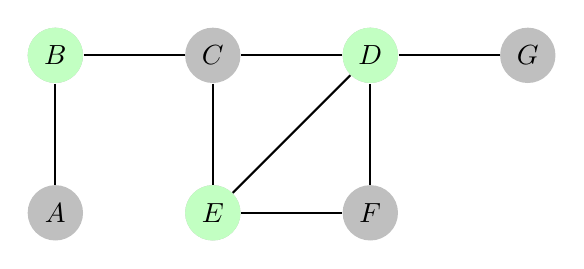
\begin{tikzpicture} [
                scale=1,
                vertex/.style={circle,fill=black!25,minimum size=20pt,inner sep=0pt},
                selected vertex/.style = {vertex, fill=green!24},
                edge/.style = {draw,thick,-},
            ]
            % First we draw the vertices
            \foreach \pos/\name in {
                    {(0,0)/A}, {(0,2)/B}, {(2,2)/C}, {(4,2)/D},
                    {(2,0)/E}, {(4,0)/F}, {(6,2)/G}}
                \node[vertex] (\name) at \pos {$\name$};
            % Connect vertices with edges and draw weights
            \foreach \source/ \dest in {
                    A/B, B/C, C/E, C/D, E/F, D/E, D/G, F/D}
                \path[edge] (\source) -- (\dest);
            % color a node
            \foreach \vertex in {B, D, E}
                \path node[selected vertex] at (\vertex) {$\vertex$};
        \end{tikzpicture}
    \end{subfigure}
    \quad
    %%%%%%%%%%%%%%%%%%%%%%%%%%%%%%%%%%%%%%%%%%%%%%%%%%%%%%%%%%%%%%%%%%%%%%%%%%%%%%%%%%%%%
    \begin{subfigure}[b]{0.45\textwidth}
        \centering
        \caption{Primo arco: $V' = \left\{ B,C \right\}$}
        \label{fig:vcapproxbad1}
        \begin{tikzpicture} [
                scale=1,
                vertex/.style={circle,fill=black!25,minimum size=20pt,inner sep=0pt},
                selected vertex/.style = {vertex, fill=blue!24},
                edge/.style = {draw,thick,-},
                selected edge/.style = {draw,line width=5pt,-,blue!35},
                ignored edge/.style = {draw,line width=5pt,-,red!25}
            ]
            % First we draw the vertices
            \foreach \pos/\name in {
                    {(0,0)/A}, {(0,2)/B}, {(2,2)/C}, {(4,2)/D},
                    {(2,0)/E}, {(4,0)/F}, {(6,2)/G}}
                \node[vertex] (\name) at \pos {$\name$};
            % Connect vertices with edges and draw weights
            \foreach \source/ \dest in {
                    A/B, B/C, C/E, C/D, E/F, D/E, D/G, F/D}
                \path[edge] (\source) -- (\dest);
            % color a node
            \foreach \vertex in {B, C}
                \path node[selected vertex] at (\vertex) {$\vertex$};
            \begin{pgfonlayer}{background}
                \foreach \source / \dest in {B/C}
                    \path[selected edge] (\source.center) -- (\dest.center);
                \foreach \source / \dest in {A/B,C/E,C/D}
                    \path[ignored edge] (\source.center) -- (\dest.center);
            \end{pgfonlayer}
        \end{tikzpicture}
    \end{subfigure}
    \\[2pt]
    %%%%%%%%%%%%%%%%%%%%%%%%%%%%%%%%%%%%%%%%%%%%%%%%%%%%%%%%%%%%%%%%%%%%%%%%%%%%%%%%%%%%%
    \begin{subfigure}[b]{0.45\textwidth}
        \centering
        \caption{Secondo arco $V' = \left\{ B,C,E,F \right\}$}
        \label{fig:vcapproxbad2}
        \begin{tikzpicture} [
                scale=1,
                vertex/.style={circle,fill=black!25,minimum size=20pt,inner sep=0pt},
                selected vertex/.style = {vertex, fill=blue!24},
                edge/.style = {draw,thick,-},
                selected edge/.style = {draw,line width=5pt,-,blue!35},
                ignored edge/.style = {draw,line width=5pt,-,red!25}
            ]
            % First we draw the vertices
            \foreach \pos/\name in {
                    {(0,0)/A}, {(0,2)/B}, {(2,2)/C}, {(4,2)/D},
                    {(2,0)/E}, {(4,0)/F}, {(6,2)/G}}
                \node[vertex] (\name) at \pos {$\name$};
            % Connect vertices with edges and draw weights
            \foreach \source/ \dest in {
                    A/B, B/C, C/E, C/D, E/F, D/E, D/G, F/D}
                \path[edge] (\source) -- (\dest);
            % color a node
                \foreach \vertex in {B, C, E, F}
                \path node[selected vertex] at (\vertex) {$\vertex$};
            \begin{pgfonlayer}{background}
                \foreach \source / \dest in {E/F}
                    \path[selected edge] (\source.center) -- (\dest.center);
                \foreach \source / \dest in {B/C,A/B,C/E,C/D,D/E,D/F}
                    \path[ignored edge] (\source.center) -- (\dest.center);
            \end{pgfonlayer}
        \end{tikzpicture}
    \end{subfigure}
    \quad
    %%%%%%%%%%%%%%%%%%%%%%%%%%%%%%%%%%%%%%%%%%%%%%%%%%%%%%%%%%%%%%%%%%%%%%%%%%%%%%%%%%%%
    \begin{subfigure}[b]{0.45\textwidth}
        \centering
        \caption{Terzo arco $V' = \left\{ B,C,E,F,D,G \right\}$}
        \label{fig:vcapproxbad3}
        \begin{tikzpicture} [
                scale=1,
                vertex/.style={circle,fill=black!25,minimum size=20pt,inner sep=0pt},
                selected vertex/.style = {vertex, fill=blue!24},
                edge/.style = {draw,thick,-},
                weight/.style = {font=\small},
                selected edge/.style = {draw,line width=5pt,-,blue!35},
                ignored edge/.style = {draw,line width=5pt,-,red!25}
            ]
            % First we draw the vertices
            \foreach \pos/\name in {
                    {(0,0)/A}, {(0,2)/B}, {(2,2)/C}, {(4,2)/D},
                    {(2,0)/E}, {(4,0)/F}, {(6,2)/G}}
                \node[vertex] (\name) at \pos {$\name$};
            % Connect vertices with edges and draw weights
            \foreach \source/ \dest in {
                    A/B, B/C, C/E, C/D, E/F, D/E, D/G, F/D}
                \path[edge] (\source) -- (\dest);
            % color a node
            \foreach \vertex in {B, C, E, F, D, G}
                \path node[selected vertex] at (\vertex) {$\vertex$};
            \begin{pgfonlayer}{background}
                \foreach \source / \dest in {D/G}
                    \path[selected edge] (\source.center) -- (\dest.center);
                \foreach \source / \dest in {B/C,E/F,A/B,C/E,C/D,D/E,D/F}
                    \path[ignored edge] (\source.center) -- (\dest.center);
            \end{pgfonlayer}
        \end{tikzpicture}
    \end{subfigure}
\end{figure}

\subsubsection{Approssimazione di $CLIQUE$}

Seguendo la funzione trovata nella riduzione da $CLIQUE$ a $VC$, si potrebbe pensare di utilizzare il risultato ottenuto per identificare una Clique nel grafo.

\begin{algorithm}[H]
\caption{Approssimatore per Clique}\label{alg:approxclique}
\begin{algorithmic}[1]
    \Procedure{Approx\_C}{$G=(V,E)$}
        \State $G^C = (V,E^C)$
        \State $V' \gets $ \Call{Approx\_VC}{$G^C$}
        \State return $V - V'$
    \EndProcedure
\end{algorithmic}
\end{algorithm}

\begin{figure}[h]
    \centering
    \caption{Trasformazione da \emph{Vertex Cover} a Clique}
    \label{fig:approxclique}
    %%%%%%%%%%%%%%%%%%%%%%%%%%%%%%%%%%%%%%%%%%%%%%%%%%%%%%%%%%%%%%%%%%%%%%%%%%%%%%%%%%%%%
    \begin{subfigure}[b]{0.3\textwidth}
        \centering
        \caption{Grafo originale}
        \label{fig:approxclique1}
        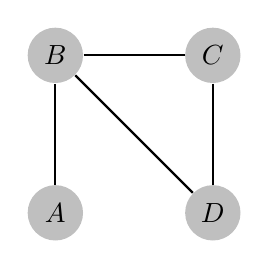
\begin{tikzpicture} [
                scale=1,
                vertex/.style={circle,fill=black!25,minimum size=20pt,inner sep=0pt},
                edge/.style = {draw,thick,-},
            ]
            % First we draw the vertices
            \foreach \pos/\name in {
                    {(0,0)/A}, {(0,2)/B}, {(2,2)/C}, {(2,0)/D}}
                \node[vertex] (\name) at \pos {$\name$};
            % Connect vertices with edges and draw weights
            \foreach \source/ \dest in {
                    A/B, B/C, C/D, B/D}
                \path[edge] (\source) -- (\dest);
        \end{tikzpicture}
    \end{subfigure}
    \quad
    %%%%%%%%%%%%%%%%%%%%%%%%%%%%%%%%%%%%%%%%%%%%%%%%%%%%%%%%%%%%%%%%%%%%%%%%%%%%%%%%%%%%%
    \begin{subfigure}[b]{0.3\textwidth}
        \centering
        \caption{$VC$ in $G^C$}
        \label{fig:approxclique2}
        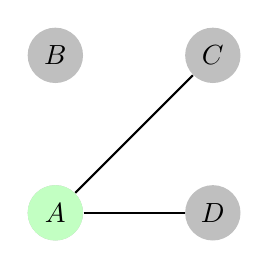
\begin{tikzpicture} [
                scale=1,
                vertex/.style={circle,fill=black!25,minimum size=20pt,inner sep=0pt},
                selected vertex/.style = {vertex, fill=green!24},
                edge/.style = {draw,thick,-},
            ]
            % First we draw the vertices
            \foreach \pos/\name in {
                    {(0,0)/A}, {(0,2)/B}, {(2,2)/C}, {(2,0)/D}}
                \node[vertex] (\name) at \pos {$\name$};
            % Connect vertices with edges and draw weights
            \foreach \source/ \dest in {
                    A/C, A/D}
                \path[edge] (\source) -- (\dest);
            % color a node
            \foreach \vertex in {A}
                \path node[selected vertex] at (\vertex) {$\vertex$};
        \end{tikzpicture}
    \end{subfigure}
    \quad
    %%%%%%%%%%%%%%%%%%%%%%%%%%%%%%%%%%%%%%%%%%%%%%%%%%%%%%%%%%%%%%%%%%%%%%%%%%%%%%%%%%%%
    \begin{subfigure}[b]{0.3\textwidth}
        \centering
        \caption{Clique in $G$}
        \label{fig:approxclique3}
        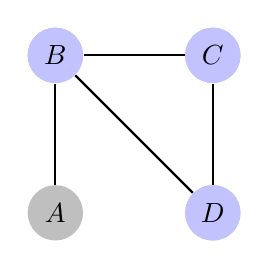
\begin{tikzpicture} [
                scale=1,
                vertex/.style={circle,fill=black!25,minimum size=20pt,inner sep=0pt},
                selected vertex/.style = {vertex, fill=blue!24},
                edge/.style = {draw,thick,-},
            ]
            % First we draw the vertices
            \foreach \pos/\name in {
                    {(0,0)/A}, {(0,2)/B}, {(2,2)/C}, {(2,0)/D}}
                \node[vertex] (\name) at \pos {$\name$};
            % Connect vertices with edges and draw weights
            \foreach \source/ \dest in {
                    A/B, B/C, C/D, B/D}
                \path[edge] (\source) -- (\dest);
            % color a node
            \foreach \vertex in {B, C, D}
                \path node[selected vertex] at (\vertex) {$\vertex$};
        \end{tikzpicture}
    \end{subfigure}
\end{figure}
Questo vale se il \emph{Vertex Cover} trovato è di dimesione massima. Se però si considera un'istanza di $CLIQUE$ $G=(V,E)$,
per cui la clique massima ha dimensione $|V^*|=n/2+1$, il $VC$ nel complementato avrà taglia $n-\left( n/2 +1 \right) = n/2 -1$. L'algoritmo di approssimazione sbaglia al massimo di un fattore 2, per cui $|V'|=2 \cdot \left( n/2 -1 \right) = n-2$. La clique trovata ha taglia $|V-V'|=n-\left( n-2 \right) = 2$. Il fattore di approssimazione risulta allora
\begin{equation*}
    \rho_{AC} \geq \frac{n/2+1}{2} \approx \frac{n}{4}
\end{equation*}
Questa cattiva prestazione dell'algoritmo deriva dal fatto che la trasformazione non preserva l'approssimazione.

% TODO pag 48 disegni strani delle riduzioni

\section{Travelling Salesman Problem}
% pag 48
Si ricordano le definizioni dei problemi di $HAMILTON$ e $TSP$:
\begin{align*}
    \text{Hamilton:} & \quad \\
    \texttt{istanza:} \quad & \langle G=(V,E) \rangle \\
    \texttt{domanda:} \quad & G \text{ contiene un ciclo semplice che tocca tutti i nodi (\emph{tour})?} \\
    \text{TSP:} & \quad \\
    \texttt{istanza:} \quad & \langle G_C=(V,E_C), c, k \rangle \\
    \text{dove} \quad & G_C \text{ grafo completo non orientato} \\
    & c : V \times V = E \to \mathbb{N} \\
    & k \in \mathbb{N} \\
    \texttt{domanda:} \quad & G \text{ contiene un ciclo \emph{Hamiltoniano} di costo $\leq k$?} \\
    \text{dove} \quad &  c(\langle v_1, \cdots, v_{|V|+1} \rangle) = \sum_{i=1}^{|V|} c(v_i, v_{i+1} )  \\
\end{align*}

\subsection{Inapprossimabilità del $TSP$ generale}
% pag 49
Se $\bp = \bnp$ sarebbe disponibile la soluzione esatta.

Sotto l'ipotesi $\bp \ne \bnp$, si mostra che se $TSP$ fosse $\rho(n)$-approssimabile in tempo polinomiale, si potrebbe risolvere un problema $\bnpc$ in tempo polinomiale, che è assurdo.

\begin{theorem}[Inapprossimabilità del $TSP$]
    \label{teo:inapprossimabilitatsp}
    Sotto l'ipotesi $\bp \ne \bnp$,
    data un'istanza di $TSP$
    $
        \langle
            G = (V,E), c
        \rangle
    $, per qualsiasi
    $
        \rho (|V|)
    $ calcolabile in tempo polinomiale,
    allora il $TSP$ non è $
        \rho (|V|)
    $-approssimabile in tempo polinomiale.
\end{theorem}
Nota: per alleggerire la notazione, $\rho \equiv \rho(|V|)$
\begin{proof}
    Per assurdo, esista un algoritmo $
    A_{TSP} ( \langle G = c \rangle)
    $ di
    $\rho$-approssimazione, poliomiale.
    Si può usare questo algoritmo per risolvere $HAMILTON$.
    Si trasforma un'istanza di $HAMILTON$ in una di $TSP$, che può essere mandata in input ad $A_{TSP}$, in maniera simile alla riduzione già vista.
    \begin{equation*}
        f :
        \langle
            G = (V,E)
        \rangle
        \to
        \langle
            G^K = (V,E^K), c
        \rangle
    \end{equation*}
    dove il grafo $G^K$ è il grafo completato, e i costi sono associati agli archi nella maniera seguente:
    \begin{equation*}
         c(e) = 
        \begin{cases}
            1 & e \in E \\
            \rho \cdot |V| & e \notin E
        \end{cases}
    \end{equation*}
    Questa funzione è calcolabile in tempo polinomiale, infatti
    \begin{itemize}[parsep=0pt,partopsep=0pt,topsep=2pt]
        \item la taglia della nuova istanza è polinomiale, il grafo completo ha numero di archi quadratico
        \item i costi sono legati a $\rho$, che è polinomiale per ipotesi, $|\rho| = poly (|V|)$
    \end{itemize}

    ``$\Rightarrow$''
    Se $ \langle G = (V,E) \rangle \in HAMILTON$, esiste in $G$ un cammino Hamiltoniano, che esiste anche in $G^K$ e ha costo $|V|$, perché tutti gli archi utilizzati sono originali.
    \\
    $A_{\rho} ( \langle G^K ,  c \rangle)$ deve ritornare un tour che non costi più di $\rho \cdot |V|$, perché è di $\rho $-approssimazione.
    Questo costo è inferiore al costo di ogni arco spurio, quindi l'algoritmo non può selezionarne nessuno.
    \\
    $A_{\rho} ( \langle G^K ,  c \rangle)$ ritorna quindi un circuito Hamiltoniano di $G$, di costo $ \leq \rho \cdot |V| + 1 $.

    ``$\Leftarrow$''
    L'algoritmo deve anche riconoscere quando un'istanza è negativa.
    \\
    $ \langle G = (V,E) \rangle \notin HAMILTON$ implica che ogni tour in $G^K$ deve usare almeno un arco in $E^K-E$.
    Allora, per ogni tour $\pi$, $c(\pi) \geq 
    \rho \cdot |V|
    + 1
    $.
    Ossia 
    $A_{\rho} ( \langle G^K ,  c \rangle)$ ritorna un tour di costo $ \geq \rho \cdot |V| + 1 $, e quindi, combinando i due risultati:
    \begin{equation*}
        \langle G \rangle \in HAMILTON
        \Leftrightarrow
        A_{\rho} ( f ( \langle G \rangle) ) \text{ ritorna un tour di costo } \leq \rho \cdot |V| + 1 
    \end{equation*}
    Sia $A_{\rho}$ sia $f$ sono polinomiali, quindi la loro composizione è polinomiale, e si è esibito un decisore per $HAMILTON$ polinomiale, che è in contrasto con l'ipotesi $\bp \ne \bnp$.
\end{proof}

\subsection{Risultati di inapprossimabilità}
% pag 50
L'idea del procedimento da seguire per provare l'inapprossimabilità di un problema è quella di creare un \emph{gap} tra il costo ottimo di istanze \emph{associate} a istanze positive e negative di un problema $\bnpc$.

Sia $\bpi_{m} \subseteq \bi \times \bs$ un problema di minimo di cui si vuole provare l'inapprossimabilità e $\bpi_{d} \in \bnpc$ un problema decisionale.
\\
Si deve trovare una funzione calcolabile in tempo polinomiale $f(x)$ che trasforma istanze di 
$\bpi_{d}$
in istanze di
$\bpi_{m}$,
tale che esiste una funzione $k(n)$ per cui
\begin{itemize}
    \item se $x \in L_{\bpi_{d}} \Rightarrow 
        c \left( 
        s^* \left( 
        f (x) \right)\right)
        \leq k \left( 
        | f(x) |
        \right)
        $
    \item se $x \notin L_{\bpi_{d}} \Rightarrow 
        c \left( 
        s^* \left( 
        f (x) \right)\right)
        > k \left( 
        | f(x) |
        \right)
        $
\end{itemize}
Studiando il costo associato alla soluzione ottima dell'istanza di 
$\bpi_{m}$,
$f(x) \in L_{ \bpi_{m} }$
si riuscirebbe a decidere un problema $\bnpc$ in tempo polinomiale.

\section{Triangle TSP}
% pag 52

\subsection{Disuguaglianza triangolare}
% pag 51

Il problema generale del $TSP$ non è di grande utilità pratica, spesso un grafo è immerso in una metrica euclidea per cui gli archi soddisfano la disuguaglianza triangolare, ovvero i costi degli archi non possono essere arbitrari.

\begin{definition}[Disuguaglianza triangolare]
    \label{def:disuguaglianzatriangolare}
    Una funzione di costo del tipo
    $c (u,v)$
    intera, posivita, simmetrica,
    soddisfa la disuguaglianza triangolare se
    \begin{equation*}
        \forall u,v,z \in V
        \Rightarrow
        c(u,v) \leq c(u,z) + c(z,v)
    \end{equation*}
\end{definition}

Anche altri spazi metrici hanno questa proprietà, per esempio lo spazio metrico indotto dai cammini minimi in un grafo.

\begin{definition}[Shortcutting]
    \label{def:shortcutting}
    In un grafo completo dove vale la disuguaglianza triangolare, si può modificare un cammino
    \begin{equation*}
        \pi = \langle \cdots, u, z, v, \cdots \rangle
        \leadsto
        \pi' = \langle \cdots, u, v, \cdots \rangle
    \end{equation*}
    e vale
    \begin{equation*}
        c (\pi') \leq c(\pi)
    \end{equation*}
    Questa proprietà si dice \emph{shortcutting} (scorciatoia).
\end{definition}

\subsection{Riduzione da TSP a TRIANGLE\_TSP}
% pag 52
Si modifica il problema del $TSP$ nel problema
$TRIANGLE\_TSP$:

\begin{align*}
    \text{TRIANGLE\_TSP:} & \quad \\
    \texttt{istanza:} \quad & \langle G=(V,E^K), c, k \rangle \\
    \text{dove} \quad & G \text{ grafo completo non orientato} \\
    & c : V \times V \to \mathbb{N} \text{ soddisfa la disuguaglianza triangolare}\\
    & k \in \mathbb{N} \\
    \texttt{domanda:} \quad & G \text{ contiene un ciclo \emph{Hamiltoniano} di costo $\leq k$?}
\end{align*}
Questa è una restrizione di un problema $\bnpc$, è stato ristretto così tanto da diventare polinomiale?
\begin{proof}[Dimostrazione $TSP \lp TRIANGLE\_TSP$]
    La funzione $f$ trasforma istanze del $TSP$ generale in istanze in cui la funzione costo rispetta la disuguaglianza triangolare scalando tutti i costi di una costante additiva.
    \begin{align*}
        f :
        \langle
        G = (V,E^K), c, k
        \rangle
        \to
        &
        \langle
        G = (V,E^K), c', k'
        \rangle
        \\
        W
        % &= 
        =
        \max_{e \in E^K} \left\{ c \left( e \right) \right\}
        ,
        \quad
        % \\
        \forall e \in E^K
        \quad
        &
        c'(e)
        =
        c(e) + W
    \end{align*}
    Questa funzione 
    \begin{itemize}
        \item è calcolabile in tempo polinomiale: $W$ è parte dell'istanza (che è polinomiale), e si somma il valore su $n^2$ archi.
        \item soddisfa la disuguaglianza triangolare:
            \begin{align*}
                \forall u,v,z
                \quad
                c'(u,v)
                &= 
                c(u,v) + W
                \\
                & \leq
                W + W
                \\
                & \leq
                c(u,z) + W + c(z,v) + W
                \\
                & \leq
                c'(u,z) + c'(z,v)
            \end{align*}
        \item è una riduzione:
            ogni tour di costo $T$ in
            $G=(V,E^K)$
            sotto $c$ diventa un tour di costo $T + |V| W$ in 
            $G=(V,E^K)$ sotto $c'$ e viceversa.
            Ogni tour infatti ha esattamente $|V|$ archi, quindi a prescindere dai loro costi singoli il costo del tour varia di $|V|W$.
            $G$ ha un tour di costo $\leq k$ sotto $c$
            se e solo se 
            $G$ ha un tour di costo $\leq k +|V|W$ sotto $c'$.
            La funzione viene specificata completamente definendo $k' = k + |V|W$.
            \begin{equation*}
                f :
                \langle
                G = (V,E^K), c, k
                \rangle
                \to
                \langle
                G = (V,E^K), c', k+|V|W
                \rangle
            \end{equation*}
            E si è mostrato che
            \begin{equation*}
                \langle
                G, c, k
                \rangle
                \in TSP
                \Leftrightarrow
                \langle
                G, c', k+|V|W
                \rangle
                \in T\_TSP
            \end{equation*}
                Per cui $T\_TSP \in \bnpc$.
    \end{itemize}
\end{proof}

\subsection{Algoritmo di 2-approssimazione per  TRIANGLE\_TSP}
\label{sss:ttsp2approx}
% pag 53-59

\subsubsection{Albero di copertura minimo}
% MST, pag 53
\begin{definition}[Albero di copertura]
    \label{def:alberocopertura}
    Dato un grafo
    $G=(V,E)$
    non orientato, connesso, un albero di copertura è un suo sottografo 
    $T_G=(V,E_G)$
    con $|E_G|=|V|-1$ e $T_G$ connesso.
\end{definition}

\begin{definition}[Albero di copertura minimo]
    \label{def:alberocoperturaminimo}
    Sotto la funzione di costo
    \begin{equation*}
        c\left( T_G \right) = 
        \sum_{e \in E_T}^{} c(e)
    \end{equation*}
    L'albero di copertura minimo (\emph{Minimum Spanning Tree}) è l'albero di copertura di $G$ di costo minimo.
\end{definition}

% Prim, pag 53
L'albero di copertura minimo si trova in tempo polinomiale, per esempio usando l'algoritmo di $Prim$ \cite{Prim57}, con complessità $O \left( |E| \log |V| \right)$, quasi lineare nel numero di archi.
\begin{enumerate}[noitemsep,parsep=0pt,partopsep=0pt,topsep=0pt]
    \item si seleziona un nodo a caso
    \item si trovano gli archi uscenti
    \item si seleziona l'arco di peso minore
    \item si itera dal punto 2 fino a toccare tutti i nodi
\end{enumerate}

\subsubsection{(Full) Preorder Walk}
% Preorder, pag 54
La visita in preordine dell'albero è chiaramente lineare nel numero di nodi
\begin{algorithm}[H]
\caption{Preorder Walk}\label{alg:preorderwalk}
\begin{algorithmic}[1]
    \Procedure{Preorder\_Visit}{$T,r$}
        \State \Call{Print}{$r$}
        \If{not (leaf (r))}
        \Comment{il nodo corrente ha figli}
        \ForAll{$v \in r.children$}
        % \Comment{RECURSE}
            \State \Call{Preorder\_Visit}{$T,v$}
        \EndFor
        \EndIf
    \EndProcedure
\end{algorithmic}
\end{algorithm}

% Full Preorder, pag 54
La visita in preordine completa (\emph{Full Preorder Visit}) si effettua stampando di nuovo il nodo quando si è conclusa l'esplorazione del sottoalbero corrispondente.
\begin{algorithm}[H]
\caption{Full Preorder Walk}\label{alg:fullpreorderwalk}
\begin{algorithmic}[1]
    \Procedure{Full\_Preorder\_Walk}{$T,r$}
        \State \Call{Print}{$r$}
        \If{not (leaf (r))}
        \ForAll{$v \in r.children$}
            \State \Call{Full\_Preorder\_Walk}{$T,v$}
            \State \Call{Print}{$r$}
        \EndFor
        \EndIf
    \EndProcedure
\end{algorithmic}
\end{algorithm}

Se si considera l'albero in figura \ref{fig:exalbero}, la visita in preordine risulta 
$ \pi = \langle a,b,c,d,e \rangle$,
mentre la visita in preordine completa è
$ \pi = \langle a,b,c,b,d,b,a,e,a \rangle$.

\begin{figure}[h]
    \centering
    \caption{Esempio di visita in preordine completa}
    \label{fig:expreordervisit}
    %%%%%%%%%%%%%%%%%%%%%%%%%%%%%%%%%%%%%%%%%%%%%%%%%%%%%%%%%%%%%%%%%%%%%%%%%%%%%%%%%%%%%
    \begin{subfigure}[b]{0.45\textwidth}
        \centering
        \caption{Albero d'esempio}
        \label{fig:exalbero}
        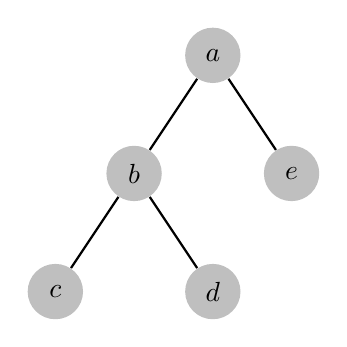
\begin{tikzpicture} [
                scale=1,
                vertex/.style={circle,fill=black!25,minimum size=20pt,inner sep=0pt},
                edge/.style = {draw,thick,-},
            ]
            \foreach \pos/\name in {
            {(0,0)/c}, {(2,0)/d}, {(1,1.5)/b}, {(3,1.5)/e}, {(2,3)/a}}
                \node[vertex] (\name) at \pos {$\name$};
            \foreach \source/ \dest in {
                    b/c,b/d,a/b,a/e}
                \path[edge] (\source) -- (\dest);
        \end{tikzpicture}
    \end{subfigure}
    %%%%%%%%%%%%%%%%%%%%%%%%%%%%%%%%%%%%%%%%%%%%%%%%%%%%%%%%%%%%%%%%%%%%%%%%%%%%%%%%%%%%%
    \begin{subfigure}[b]{0.45\textwidth}
        \centering
        \caption{$FPW$}
        \label{fig:fullpreordervisit}
        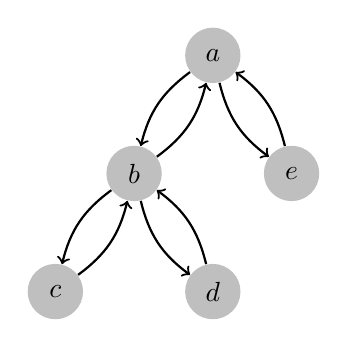
\begin{tikzpicture} [
                scale=1,
                vertex/.style={circle,fill=black!25,minimum size=20pt,inner sep=0pt},
                edge/.style = {draw,thick,-},
                arrow edge/.style = {draw,thick,->},
                bent right/.style = {bend right=20},
                bent left/.style = {bend left=20},
            ]
            \foreach \pos/\name in {
            {(0,0)/c}, {(2,0)/d}, {(1,1.5)/b}, {(3,1.5)/e}, {(2,3)/a}}
                \node[vertex] (\name) at \pos {$\name$};
            \foreach \source/ \dest in {
                    b/c,b/d,a/b,a/e}
                \path[arrow edge] (\source) edge [bent right] (\dest);
            \foreach \source/ \dest in {
                    c/b,d/b,b/a,e/a}
                \path[arrow edge] (\source) edge [bent right] (\dest);
        \end{tikzpicture}
    \end{subfigure}
\end{figure}

La visita in preordine completa forma un ciclo (non semplice) all'interno dell'albero (figura \ref{fig:fullpreordervisit}).

\begin{proposizione}
    \label{prop:costofpw}
    Il costo della $FPW$ è due volte il costo del $MST$
    \begin{equation*}
        c(FPW) = 2 \cdot c(MST)
        % = 2 \cdot c(T^*)
    \end{equation*}
    \begin{proof}
        La $FPW$ utilizza ogni arco del $MST$ esattamente due volte. La prima volta mentre sta scendendo ricorsivamente l'albero, seleziona $\left\{ r,v \right\}$, e la seconda mentre risale, selezionando $\left\{ v,r \right\}$.
    \end{proof}
\end{proposizione}

\subsubsection{Algoritmo di approssimazione}
% Approx TTSP, pag 53.8
\begin{algorithm}[H]
\caption{Approssimatore per Triangle TSP}\label{alg:approxttsp}
\begin{algorithmic}[1]
    \Procedure{Approx\_T\_TSP}{$i$}
        \State $T_G \gets$ \Call{Prim}{$ \langle G, c\rangle$}
        \State $\pi \gets$ \Call{Preorder\_Visit}{$T_G$}
        \State * sia $\pi = \langle v_1, v_2, \cdots, v_{|V|}\rangle $ *
        \State return $\langle \pi, v_1 \rangle $
    \EndProcedure
\end{algorithmic}
\end{algorithm}

Se si considera di nuovo l'albero in figura \ref{fig:exalbero}, l'algoritmo ritorna
$ \pi = \langle a,b,c,d,e,a \rangle$.

\begin{figure}[h]
    \centering
    \caption{Risultato dell'algoritmo}
    \label{fig:approxttsp2}
    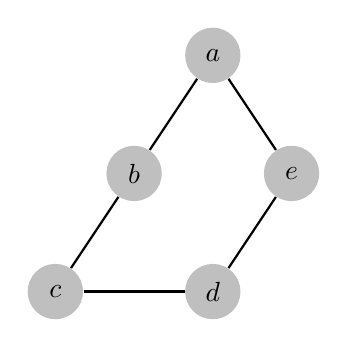
\begin{tikzpicture} [
            scale=1,
            vertex/.style={circle,fill=black!25,minimum size=20pt,inner sep=0pt},
            edge/.style = {draw,thick,-},
        ]
        \foreach \pos/\name in {
                {(0,0)/c}, {(2,0)/d}, {(1,1.5)/b}, {(3,1.5)/e}, {(2,3)/a}}
            \node[vertex] (\name) at \pos {$\name$};
        \foreach \source/ \dest in {
                b/c,c/d,a/b,a/e,d/e}
            \path[edge] (\source) edge (\dest);
    \end{tikzpicture}
\end{figure}

% Fattore approssimazione approx TTSP, pag 55
Riguardo al fattore di approssimazione di questo algoritmo, vanno trovati \emph{bound} per
\begin{equation*}
    \rho =
    \frac{
    |H'|
    }{
    |H^*|
    }
    =
    \frac{
        \text{costo soluzione ammissibile ritornata}
    }{
        \text{costo soluzione ottima}
    }
\end{equation*}
Dove si indica $H'$ la soluzione trovata al problema $T\_TSP$, $H^*$ la soluzione ottima al problema, $T^*$ il \emph{minimum spanning tree} del grafo.

\begin{itemize}
    \item Per $|H'|$: il ciclo ritornato è una sotto sequenza della \emph{full preorder walk}, dove vengono selezionati i nodi la prima volta che vengono visti (ed aggiunta la radice).
        \begin{equation*}
            H' = \langle a,b,c,d,e,a \rangle
            \quad
            FPW = \langle \underline{a},\underline{b},\underline{c},b,\underline{d},b,a,\underline{e},a \rangle
        \end{equation*}
        Per la proprietà dello \emph{shortcutting}, vale $
        c(H') \leq c(FPW)
        $
        e dalla proposizione \ref{prop:costofpw} si conosce $
        c(FPW) = 2 \, c(MST)
        = 2 \, c(T^*)
        $.
        Componendo si ottiene 
        \begin{equation*}
            c(H')
            % \leq c(FPW)
            % = 2 \cdot c(T^*)
            \leq 2 \, c(T^*)
        \end{equation*}
    \item Per $|H^*|$:
        Se dal ciclo ottimo
        $H^*$
        si rimuove un arco $e$ qualsiasi, si ottiene uno \emph{spanning tree}
        generico
        % (di costo non necessariamente minimo)
        , che è di sicuro non di costo inferiore al migliore albero di copertura trovato:
        \begin{equation*}
            c(H^*) \geq 
            c(H^* - \{ e \} ) =
            c(ST) \geq 
            c(T^*)
        \end{equation*}
\end{itemize}
Componendo i risultati
\begin{equation*}
    \rho =
    \frac{
        |H'|
    }{
        |H^*|
    }
    \leq
    \frac{
        2 \, c(T^*)
    }{
        |H^*|
    }
    \leq
    \frac{
        2 \, c(T^*)
    }{
        c(T^*)
    }
    = 2
\end{equation*}

\subsection{Algoritmo di Christofides}
% pag 56

\subsubsection{Multigrafi e circuiti Euleriani}

% multigrafo, pag 56.2
\begin{definition}[Multigrafo]
    \label{def:multigrafo}
    Un multigrafo $G=(V,E)$ non orientato è costruito su un insieme di nodi e un multiinsieme di archi.
    Ogni arco $e \in E$ può essere presente in multiple copie:
    \begin{equation*}
        \text{molteplicità:}
        \quad
        m(e) = \text{\# copie di $e$}
    \end{equation*}
    Il grado di un nodo deve tenere conto di tutte le copie degli archi incidenti:
    \begin{equation*}
        deg(v) = \sum_{e : v \in e}^{} m(e)
    \end{equation*}
    Cammini e cicli sono definiti come per un grafo.
\end{definition}

% circuito Euleriano, pag 56.5
\begin{definition}[Circuito Euleriano]
    \label{def:circuitoeuleriano}
    Un circuito Euleriano è un ciclo \emph{non semplice} che tocca tutti gli archi del grafo.
    Un (multi)grafo è Euleriano se ammette un circuito Euleriano.
\end{definition}

\begin{definition}[Grafo Euleriano]
    \label{def:grafoeuleriano}
    Un (multi)grafo è Euleriano se ammette un circuito Euleriano.
\end{definition}

% teorema di eulero, pag 56.7
\begin{theorem}
    \label{teo:grafoeuleriano}
    Un multigrafo connesso è Euleriano se e solo se tutti i vertici del grafo hanno grado pari.
\end{theorem}

% prop nodi dispari in numero pari, pag 57.5
\begin{proposizione}
    Dato un (multi)grafo non orientato, il numeri di vertici di grado dispari è sempre pari.
    \begin{proof}
        Ogni arco incide su due vertici, per cui
        \begin{equation*}
            2 |E| 
            =
            \sum_{v \in V}^{} deg(v)
            = 
            \sum_{v \in V_{EVEN}}^{} deg(v)
            +
            \sum_{v \in V_{ODD}}^{} deg(v)
        \end{equation*}
        La somma dei due termini deve essere pari,
        % Dei due termini della somma,
        il primo è pari perché somma di contributi pari,
        quindi anche il secondo deve essere pari.
        Perché una somma di contributi dispari sia pari, deve essere un numero pari di contributi.
    \end{proof}
\end{proposizione}

% def matching perfetto, pag 57.3
\begin{definition}[Matching perfetto]
    \label{def:matchingperfetto}
    Dato un grafo $G$ con $|V| = 2k$ un matching perfetto è un insieme di archi $M \subseteq E$ tale che
    \begin{itemize}
        \item $\forall e_1, e_2 \in M : e_1 \cap e_2 = \emptyset$
        \item $\forall v \in V, \exists e \in M : v \in e$
    \end{itemize}
\end{definition}
Il grafo deve avere un numero pari di nodi perché ogni arco ne copre due.
\\
Se $G$ è pesato esiste un matching perfetto di costo minimo, che può essere individuato con l'algoritmo di \emph{Gabow} in tempo $
O(|E||V|)
$, che in caso di grafo denso ($
|E| = \Theta (|V|^2)
$) diventa $
O(|V|^3)
$.

\subsubsection{Christofides}
% pag 56.9, 57.1

Christofides nel 1976 \cite{Chr76} ha trovato un algoritmo di 3/2-approssimazione per TRIANGLE\_TSP.

L'idea è di partire da un $MST$ ed aggiungere archi in modo da rendere pari ogni nodo, e poi semplificare il cammino Euleriano trovato usando lo \emph{shortcutting}, come mostrato in figura \ref{fig:christofides}.

% \begin{figure}[h]
\begin{figure}[!b]
% \begin{figure}[H]
    \centering
    \caption{Algoritmo di Christofides}
    \label{fig:christofides}
    %%%%%%%%%%%%%%%%%%%%%%%%%%%%%%%%%%%%%%%%%%%%%%%%%%%%%%%%%%%%%%%%%%%%%%%%%%%%%%%%%%%%%
    \begin{subfigure}[b]{0.45\textwidth}
        \centering
        \caption{$T^*$ con i nodi dispari evidenziati}
        \label{fig:christmst}
        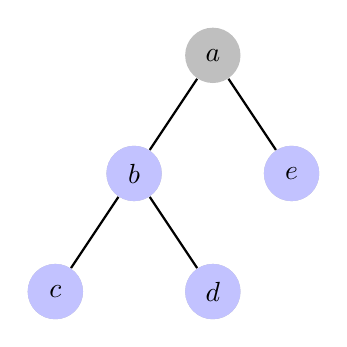
\begin{tikzpicture} [
                scale=1,
                vertex/.style={circle,fill=black!25,minimum size=20pt,inner sep=0pt},
                edge/.style = {draw,thick,-},
                selected vertex/.style = {vertex, fill=blue!24},
            ]
            \foreach \pos/\name in {
                    {(0,0)/c}, {(2,0)/d}, {(1,1.5)/b}, {(3,1.5)/e}, {(2,3)/a}}
                \node[vertex] (\name) at \pos {$\name$};
            \foreach \source/ \dest in {
                    b/c,b/d,a/b,a/e}
                \path[edge] (\source) edge (\dest);
            \foreach \vertex in {b,c,d,e}
                \path node[selected vertex] at (\vertex) {$\vertex$};
        \end{tikzpicture}
    \end{subfigure}
    \quad
    %%%%%%%%%%%%%%%%%%%%%%%%%%%%%%%%%%%%%%%%%%%%%%%%%%%%%%%%%%%%%%%%%%%%%%%%%%%%%%%%%%%%%
    \begin{subfigure}[b]{0.45\textwidth}
        \centering
        \caption{Sottografo (completo) indotto dai nodi dispari, e matching perfetto di costo minimo evidenziato}
        \label{fig:christmatching}
        \begin{tikzpicture} [
                scale=1,
                vertex/.style={circle,fill=black!25,minimum size=20pt,inner sep=0pt},
                edge/.style = {draw,thick,-},
                selected edge/.style = {draw,line width=5pt,-,blue!24},
            ]
            \foreach \pos/\name in {
                    {(0,0)/c}, {(2,0)/d}, {(1,1.5)/b}, {(3,1.5)/e}}
                \node[vertex] (\name) at \pos {$\name$};
            \foreach \source/ \dest in {
                    b/c,b/d,b/e,c/e,c/d,e/d}
                \path[edge] (\source) edge (\dest);
            \begin{pgfonlayer}{background}
                \foreach \source / \dest in {b/c,d/e}
                    \path[selected edge] (\source.center) -- (\dest.center);
            \end{pgfonlayer}
        \end{tikzpicture}
    \end{subfigure}
\end{figure}
    % \\[2pt]
% magic to split a figure https://tex.stackexchange.com/a/278748
\begin{figure}[htb]\ContinuedFloat
    %%%%%%%%%%%%%%%%%%%%%%%%%%%%%%%%%%%%%%%%%%%%%%%%%%%%%%%%%%%%%%%%%%%%%%%%%%%%%%%%%%%%%
    \begin{subfigure}[b]{0.45\textwidth}
        \centering
        \caption{Ciclo Euleriano
            $ \langle c,b,d,e,a,b,c \rangle$
        }
        \label{fig:christeulertour}
        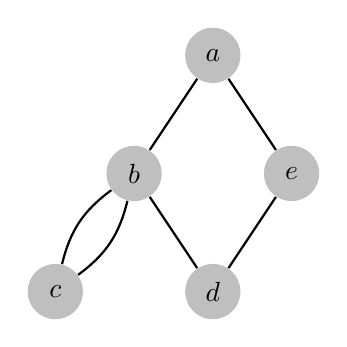
\begin{tikzpicture} [
                scale=1,
                vertex/.style={circle,fill=black!25,minimum size=20pt,inner sep=0pt},
                edge/.style = {draw,thick,-},
                bent right/.style = {bend right=20},
            ]
            \foreach \pos/\name in {
                    {(0,0)/c}, {(2,0)/d}, {(1,1.5)/b}, {(3,1.5)/e}, {(2,3)/a}}
                \node[vertex] (\name) at \pos {$\name$};
            \foreach \source/ \dest in {
                    b/d,a/b,a/e,d/e}
                \path[edge] (\source) edge (\dest);
            \foreach \source/ \dest in {
                    c/b,b/c}
                \path[edge] (\source) edge [bent right] (\dest);
        \end{tikzpicture}
    \end{subfigure}
    \quad
    %%%%%%%%%%%%%%%%%%%%%%%%%%%%%%%%%%%%%%%%%%%%%%%%%%%%%%%%%%%%%%%%%%%%%%%%%%%%%%%%%%%%%
    \begin{subfigure}[b]{0.45\textwidth}
        \centering
        \caption{Dopo lo \emph{shortcutting}:
            $ \langle c,b,d,e,a,\cancel{b},c \rangle$
        }
        \label{fig:christresult}
        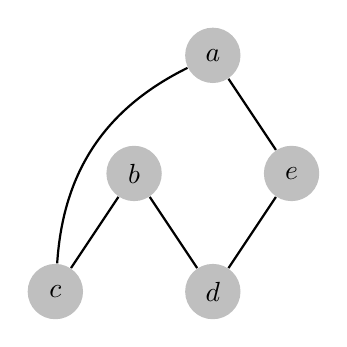
\begin{tikzpicture} [
                scale=1,
                vertex/.style={circle,fill=black!25,minimum size=20pt,inner sep=0pt},
                edge/.style = {draw,thick,-},
                bent right/.style = {bend right=30},
            ]
            \foreach \pos/\name in {
                    {(0,0)/c}, {(2,0)/d}, {(1,1.5)/b}, {(3,1.5)/e}, {(2,3)/a}}
                \node[vertex] (\name) at \pos {$\name$};
            \foreach \source/ \dest in {
                    b/d,a/e,d/e,b/c}
                \path[edge] (\source) edge (\dest);
            \foreach \source/ \dest in {
                    a/c}
                \path[edge] (\source) edge [bent right] (\dest);
        \end{tikzpicture}
    \end{subfigure}
\end{figure}

% Fattore approssimazione, pag 58-59.5

Il grafo ottenuto (prima dello \emph{shortcutting}), è
\begin{equation*}
    G' = 
    (
        V, \,
        E_{T^*}
        \cup
        M^*
    )
\end{equation*}
È già stato mostrato nella sezione \ref{sss:ttsp2approx} che
$ c(T^*) \leq c(H^*) $.
Resta da dimostrare che
% \begin{equation*}
$
    c( M^*)
    \leq
    % \frac{c\left( H^* \right)}{2}
    c\left( H^* \right) / 2
% \end{equation*}
$.
Si supponga di conoscere $H^*$ e di aver calcolato $T^*$. Alcuni nodi in $T^*$ saranno di grado pari \emph{in} $T^*$. Usando lo \emph{shortcutting}, si rimuovono questi nodi da $
H^*
$, ottenendo $
H^{*'}
$, con chiaramente $
c( H^{*'})
\leq
c(H^* )
$.
I nodi dispari in $T^*$ erano in numero pari, quindi $
H^{*'}
$ ha un numero pari di vertici.
Colorando in modo alternato gli archi del ciclo, gli archi di ciascun colore sono un matching: $
H^{*'}
= M_B \cup M_R
$, il cui costo è pari al costo del ciclo $
c( H^{*'}) = c(M_B) + c(M_R)
$. Combinando i due vincoli sui costi si ottiene
\begin{equation*}
    c(M_B) + c(M_R)
    \leq
    c(H^* )
\end{equation*}
Se si indica il matching di costo inferiore con $M_X$, deve valere
\begin{equation*}
    c(M_X)
    \leq
    \frac{
    c(H^* )
    }{2}
\end{equation*}
($x+y\leq z \to \min \left\{ x,y \right\} \leq z/2$).
Il matching perfetto 
costruito sui nodi dispari di $T^*$
dall'algoritmo di Christofides è quello ottimo $M^*$, di costo $
    c(M^*)
    \leq
    c(M_X)
$. Combinando,
\begin{equation*}
    c( M^*)
    \leq
    \frac{c\left( H^* \right)}{2}
\end{equation*}
In conclusione
\begin{equation*}
    c (H') \leq
    c ( E_{T^*} \cup M^*) \leq 
    c\left( H^* \right)
    +
    \frac{c\left( H^* \right)}{2}
    =
    \frac{3}{2} \,
    c\left( H^* \right)
\end{equation*}

\subsection{Altri risultati sull'approssimazione di TSP}

Arora ha mostrato nel 1998 \cite{Arora:1998:PTA:290179.290180} che $EUCLIDEAN\_TSP$ (in cui la distanza per esempio è la norma 2) ammette un algoritmo PTAS,
per cui
$
\forall \varepsilon,
\rho \leq 1+\varepsilon
$
e la complessità è $
O \left( n^{1/\varepsilon} \right)
$.

Papadimitriou e Vempala hanno mostrato nel 2006 \cite{Papadimitriou:2006:s00493-006-0008-z} che il $TRIANGLE\_TSP$ con archi simmetrici non può essere approssimato con un fattore migliore di 220/219.

\section{Set Cover}

\section{FPTAS Subset Sum}

\section{Pezzi utili di \LaTeX{}}
\begin{algorithm}[H]
\caption{Divide and Conquer}\label{alg:dnc}
\begin{algorithmic}[1]
    \Procedure{Divide\&Conquer}{$i$}
        \If{$|i| \leq n_0$}
        \Comment{BASE}
            \State *risolvo direttamente*
        \EndIf
        \State $\langle i_1, i_2, \dots, i_k \rangle \gets A_D(i)$ 
        \Comment{DIVIDE}
        \For{$j \gets 1 $ to $ k $ }
        \Comment{RECURSE}
            \State $s_j \gets $ \Call{Divide\&Conquer}{$i_j$}
        \EndFor
        \State $s \gets A_C(\langle s_1, s_2, \dots, s_k \rangle)$
        \Comment{CONQUER}
        \State return $s$
    \EndProcedure
\end{algorithmic}
\end{algorithm}
\noindent
Testo non identato!

\begin{definition}[Algoritmo]\label{def:algex}
    Un algoritmo è una procedura computazionale finita (terminante) e deterministica, specificata come una sequenza di passi elementari (istruzioni) estratte da un insieme standard associato a un modello computazionale (astrazione di un computer) che trasforma in maniera univoca un ingresso in un uscita.
\end{definition}

Guarda che so fare
\begin{equation*}
    \setzo{m}
    \quad
    \setzo{}
\end{equation*}

Un problema
\begin{align*}
    SS: & \\
    \texttt{istanza:} \quad & \langle S,t \rangle \\
    \text{dove} \quad & S \subseteq \mathbb{N} - \left\{ 0 \right\} \text{ finito} \\
    & t \subseteq \mathbb{N} - \left\{ 0 \right\} \\
    \texttt{domanda:} \quad & \exists \, S' \subseteq S : \sum_{s \in S'}^{} s = t \, ?
\end{align*}

Una lista
\begin{itemize}[noitemsep,parsep=0pt,partopsep=0pt,topsep=0pt]
    \item[--] $L_A = L$ (il linguaggio deciso da $A$ è $L$)
    \item[--] $T_A(|x|) = O(|x|^k)$ per qualche costante $k \geq 0$
\end{itemize}

\subsection{Grafi}

Grafi facili da mantenere

% Declare layers (done in main)
\pgfdeclarelayer{background}
\pgfsetlayers{background,main}

\begin{figure}[h]
    \centering
    \caption{Algoritmo di Prim}
    \label{fig:prim1}
    %%%%%%%%%%%%%%%%%%%%%%%%%%%%%%%%%%%%%%%%%%%%%%%%%%%%%%%%%%%%%%%%%%%%%%%%%%%%%%%%%%%%%
    \begin{subfigure}[b]{0.45\textwidth}
        \centering
        \caption{Archi uscenti dal primo nodo}
        \label{fig:au1}
        \begin{tikzpicture} [
                % automagically put labels not on edges
                auto,
                % exchanges the roles of left and right in automatic placement
                % the side the label is put on depends on the order of the nodes in the edge
                swap,
                scale=1.4,
                vertex/.style={circle,fill=black!25,minimum size=20pt,inner sep=0pt},
                selected vertex/.style = {vertex, fill=red!24},
                edge/.style = {draw,thick,-},
                weight/.style = {font=\small},
                selected edge/.style = {draw,line width=5pt,-,red!50},
                outbound edge/.style = {draw,line width=5pt,-,blue!50},
                ignored edge/.style = {draw,line width=5pt,-,black!20}
            ]
            % First we draw the vertices
            \foreach \pos/\name in {
                {(0,0)/d}, {(0,2)/a}, {(1.5,2)/b}, {(4,2)/c}, {(3,1.2)/e}, {(2,0)/f}, {(4,0)/g}}
                \node[vertex] (\name) at \pos {$\name$};
            % Connect vertices with edges and draw weights
            \foreach \source/ \dest /\weight in {b/a/7, c/b/8, d/a/5, d/b/9,
                                                 e/b/7, e/c/5, e/d/15,
                                                 f/d/6, f/e/8, g/e/9, g/f/11}
                \path[edge] (\source) -- node[weight] {$\weight$} (\dest);
            % color a node
            % \path node[selected vertex] at (d) {$d$};
            % prepare it in loop version anyway
            \foreach \vertex in {d}
                \path node[selected vertex] at (\vertex) {$\vertex$};
            % For convenience we use a background layer to highlight edges
            % This way we don't have to worry about the highlighting covering
            % weight labels. 
            \begin{pgfonlayer}{background}
                \foreach \source / \dest in {d/a,d/b,d/e,d/f}
                    \path[outbound edge] (\source.center) -- (\dest.center);
            \end{pgfonlayer}
        \end{tikzpicture}
    \end{subfigure}
    \quad
    %%%%%%%%%%%%%%%%%%%%%%%%%%%%%%%%%%%%%%%%%%%%%%%%%%%%%%%%%%%%%%%%%%%%%%%%%%%%%%%%%%%%%
    \begin{subfigure}[b]{0.45\textwidth}
        \centering
        \caption{Arco selezionato}
        \label{fig:au2}
        \begin{tikzpicture} [
                auto,
                swap,
                scale=1.4,
                vertex/.style={circle,fill=black!25,minimum size=20pt,inner sep=0pt},
                selected vertex/.style = {vertex, fill=red!24},
                edge/.style = {draw,thick,-},
                weight/.style = {font=\small},
                selected edge/.style = {draw,line width=5pt,-,red!50},
                outbound edge/.style = {draw,line width=5pt,-,blue!50},
                ignored edge/.style = {draw,line width=5pt,-,black!20}
            ]
            % First we draw the vertices
            \foreach \pos/\name in {
                {(0,0)/d}, {(0,2)/a}, {(1.5,2)/b}, {(4,2)/c}, {(3,1.2)/e}, {(2,0)/f}, {(4,0)/g}}
                \node[vertex] (\name) at \pos {$\name$};
            % Connect vertices with edges and draw weights
            \foreach \source/ \dest /\weight in {b/a/7, c/b/8, d/a/5, d/b/9,
                                                 e/b/7, e/c/5, e/d/15,
                                                 f/d/6, f/e/8, g/e/9, g/f/11}
                \path[edge] (\source) -- node[weight] {$\weight$} (\dest);
            % color a node
            \foreach \vertex in {d,a}
                \path node[selected vertex] at (\vertex) {$\vertex$};
            \begin{pgfonlayer}{background}
                \foreach \source / \dest in {b/a,d/b,d/e,d/f}
                    \path[outbound edge] (\source.center) -- (\dest.center);
                \foreach \source / \dest in {d/a}
                    \path[selected edge] (\source.center) -- (\dest.center);
            \end{pgfonlayer}
        \end{tikzpicture}
    \end{subfigure}
    \\[2pt]
    %%%%%%%%%%%%%%%%%%%%%%%%%%%%%%%%%%%%%%%%%%%%%%%%%%%%%%%%%%%%%%%%%%%%%%%%%%%%%%%%%%%%%
    \begin{subfigure}[b]{0.45\textwidth}
        \centering
        \caption{Secondo arco selezionato}
        \label{fig:au3}
        \begin{tikzpicture} [
                auto,
                swap,
                scale=1.4,
                vertex/.style={circle,fill=black!25,minimum size=20pt,inner sep=0pt},
                selected vertex/.style = {vertex, fill=red!24},
                edge/.style = {draw,thick,-},
                weight/.style = {font=\small},
                selected edge/.style = {draw,line width=5pt,-,red!50},
                outbound edge/.style = {draw,line width=5pt,-,blue!50},
                ignored edge/.style = {draw,line width=5pt,-,black!20}
            ]
            % First we draw the vertices
            \foreach \pos/\name in {
                {(0,0)/d}, {(0,2)/a}, {(1.5,2)/b}, {(4,2)/c}, {(3,1.2)/e}, {(2,0)/f}, {(4,0)/g}}
                \node[vertex] (\name) at \pos {$\name$};
            % Connect vertices with edges and draw weights
            \foreach \source/ \dest /\weight in {b/a/7, c/b/8, d/a/5, d/b/9,
                                                 e/b/7, e/c/5, e/d/15,
                                                 f/d/6, f/e/8, g/e/9, g/f/11}
                \path[edge] (\source) -- node[weight] {$\weight$} (\dest);
            % color a node
            \foreach \vertex in {d,a}
                \path node[selected vertex] at (\vertex) {$\vertex$};
            \begin{pgfonlayer}{background}
                \foreach \source / \dest in {b/a,d/b,d/e,e/f,f/g}
                    \path[outbound edge] (\source.center) -- (\dest.center);
                \foreach \source / \dest in {d/a, d/f}
                    \path[selected edge] (\source.center) -- (\dest.center);
            \end{pgfonlayer}
        \end{tikzpicture}
    \end{subfigure}
    \quad
    %%%%%%%%%%%%%%%%%%%%%%%%%%%%%%%%%%%%%%%%%%%%%%%%%%%%%%%%%%%%%%%%%%%%%%%%%%%%%%%%%%%%%
    \begin{subfigure}[b]{0.45\textwidth}
        \centering
        \caption{Terzo arco selezionato, notare il primo arco ignorato, interno al $MST$.
            La subcaption può essere lunga assai, e brutte cose non succedono
        }
        \label{fig:au4}
        \begin{tikzpicture} [
                auto,
                swap,
                scale=1.4,
                vertex/.style={circle,fill=black!25,minimum size=20pt,inner sep=0pt},
                selected vertex/.style = {vertex, fill=red!24},
                edge/.style = {draw,thick,-},
                weight/.style = {font=\small},
                selected edge/.style = {draw,line width=5pt,-,red!50},
                outbound edge/.style = {draw,line width=5pt,-,blue!50},
                ignored edge/.style = {draw,line width=5pt,-,black!20}
            ]
            % First we draw the vertices
            \foreach \pos/\name in {
                {(0,0)/d}, {(0,2)/a}, {(1.5,2)/b}, {(4,2)/c}, {(3,1.2)/e}, {(2,0)/f}, {(4,0)/g}}
                \node[vertex] (\name) at \pos {$\name$};
            % Connect vertices with edges and draw weights
            \foreach \source/ \dest /\weight in {b/a/7, c/b/8, d/a/5, d/b/9,
                                                 e/b/7, e/c/5, e/d/15,
                                                 f/d/6, f/e/8, g/e/9, g/f/11}
                \path[edge] (\source) -- node[weight] {$\weight$} (\dest);
            % color a node
            \foreach \vertex in {d,a}
                \path node[selected vertex] at (\vertex) {$\vertex$};
            \begin{pgfonlayer}{background}
                \foreach \source / \dest in {d/b,d/e,e/f,f/g,b/e,b/c}
                    \path[outbound edge] (\source.center) -- (\dest.center);
                \foreach \source / \dest in {d/a, d/f, a/b}
                    \path[selected edge] (\source.center) -- (\dest.center);
                \foreach \source / \dest in {d/b}
                    \path[ignored edge] (\source.center) -- (\dest.center);
            \end{pgfonlayer}
        \end{tikzpicture}
    \end{subfigure}
\end{figure}

\begin{figure}[h]
    \centering
    \caption{Unweighted graph}
    \label{fig:ug}
    \begin{tikzpicture} [
            auto,
            swap,
            scale=1.4,
            vertex/.style={circle,fill=black!25,minimum size=20pt,inner sep=0pt},
            selected vertex/.style = {vertex, fill=red!24},
            edge/.style = {draw,thick,-},
            weight/.style = {font=\small},
            selected edge/.style = {draw,line width=5pt,-,red!50},
            outbound edge/.style = {draw,line width=5pt,-,blue!50},
            ignored edge/.style = {draw,line width=5pt,-,black!20}
        ]
        % First we draw the vertices
        \foreach \pos/\name in {
                {(0,0)/A},
                {(0,2)/B},
                {(2,2)/C},
                {(4,2)/D},
                {(2,0)/E},
                {(4,0)/F},
                {(6,2)/G}}
            \node[vertex] (\name) at \pos {$\name$};
        % Connect vertices with edges and draw weights
        \foreach \source/ \dest in {
                A/B, B/C, C/E, C/D, E/F, D/E, D/G, F/D}
            \path[edge] (\source) -- (\dest);
        % color a node
        \foreach \vertex in {B, D, E}
            \path node[selected vertex] at (\vertex) {$\vertex$};
        \begin{pgfonlayer}{background}
            \foreach \source / \dest in {B/C}
                \path[outbound edge] (\source.center) -- (\dest.center);
            \foreach \source / \dest in {D/G}
                \path[selected edge] (\source.center) -- (\dest.center);
            \foreach \source / \dest in {F/D}
                \path[ignored edge] (\source.center) -- (\dest.center);
        \end{pgfonlayer}
    \end{tikzpicture}
\end{figure}

\begin{figure}[h]
    \centering
    \caption{$FPW$}
    \label{fig:exbend}
    \begin{tikzpicture} [
            scale=1.4,
            vertex/.style={circle,fill=black!25,minimum size=20pt,inner sep=0pt},
            edge/.style = {draw,thick,-},
            outbound edge/.style = {draw,line width=8pt,-,blue!30},
            selected edge/.style = {draw,line width=8pt,-,red!30},
            arrow edge/.style = {draw,thick,->},
            bent right/.style = {bend right=20},
            bent left/.style = {bend left=20},
        ]
        \foreach \pos/\name in {
        {(0,0)/c}, {(2,0)/d}, {(1,1.5)/b}, {(3,1.5)/e}, {(2,3)/a}}
            \node[vertex] (\name) at \pos {$\name$};
        \foreach \source/ \dest in {
                b/c,b/d,a/b,a/e}
            \path[arrow edge] (\source) edge [bent right] (\dest);
        \foreach \source/ \dest in {
                c/b,d/b,b/a,e/a}
            \path[arrow edge] (\source) edge [bent right] (\dest);
        \begin{pgfonlayer}{background}
            \foreach \source / \dest in {a/b}
                \path[outbound edge] (\source) edge [bent right] (\dest);
            \foreach \source / \dest in {b/a}
                \path[selected edge] (\source) edge [bent right] (\dest);
        \end{pgfonlayer}
    \end{tikzpicture}
\end{figure}
